\documentclass[12pt]{beamer}
\usetheme{Frankfurt}
\usepackage[utf8x]{inputenc}
\usepackage{ucs}
\usepackage{amsmath}
\usepackage{amsfonts}
\usepackage{amssymb}
\usepackage{graphicx}
\author{Bruce Nolasco}
\title{Presentación 1}
%\setbeamercovered{transparent} 
%\setbeamertemplate{navigation symbols}{} 
%\logo{} 
\institute{Facultad de Ciencias UNAM} 
\date{1 de Octubre del 2017 } 
\subject{Computación para Físicos} 
\begin{document}

\begin{frame}
\titlepage
\end{frame}

\begin{frame}
\tableofcontents
\end{frame}

%\chapter{Capítulo 1}
\section{Tema 1: LaTeX}
\begin{frame}{Diapositiva 1}

Cómo construir documentos en LaTeX. \\

\textbf{Las ecuaciones} \textit{van entre signos} \$.

\emph{Las tortillas valen} \$ 13 el kilo.

\begin{equation}
\frac{\sin{3\theta}}{\cos {2x}}
\end{equation}

\end{frame}
\subsection{Subtema LaTeX}
\begin{frame}
Iniciar presentaciones en Beamer hechas con \LaTeX
\end{frame}

\section{Tema 2: Integrales}
\begin{frame}{Integrales}


\begin{equation}
\displaystyle \int_{\alpha_{1}}^{\alpha_{2}} \Sigma_{n=1}^{\infty} n \cdot x dx
\end{equation}
\begin{equation}
\int_{\alpha_{1}}^{\alpha_{2}} \Sigma_{n=1}^{\infty} n \cdot x dx
\end{equation}
\begin{equation}
\displaystyle \int_{\alpha_{1}}^{\alpha_{2}} 
\displaystyle \sum_{n=1}^{\infty} n \cdot x dx
\end{equation}

\end{frame}

\subsection{Imagenes}

\begin{frame}{Diapositiva de Imagen}
\begin{figure}[t]
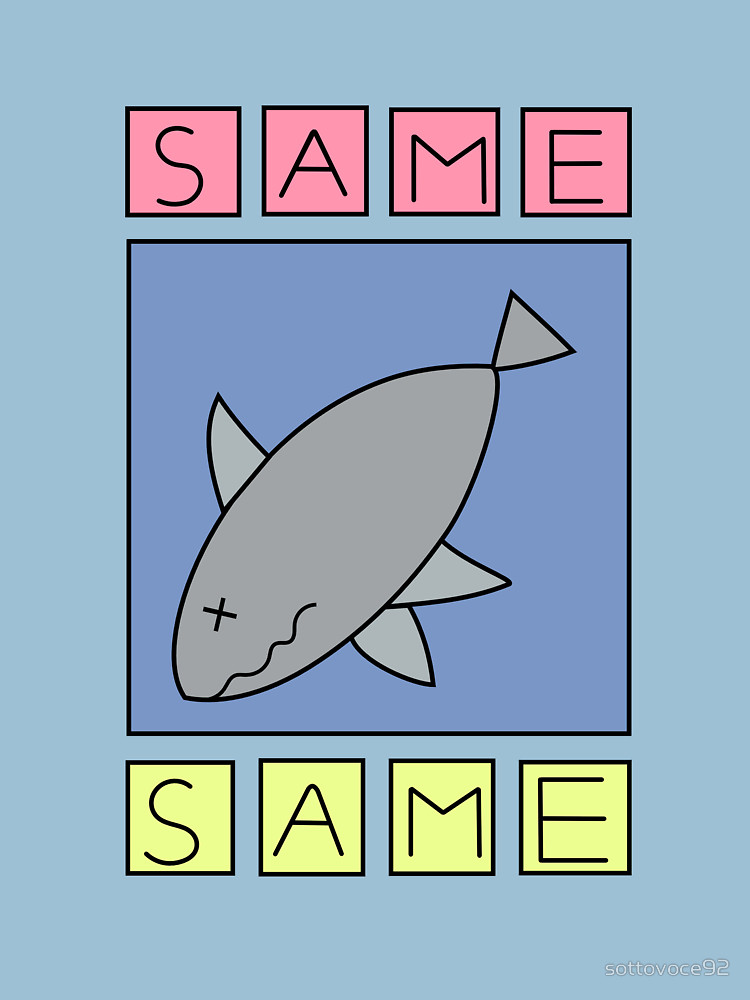
\includegraphics[scale=0.15]{shark.jpg} 
\caption{Imagen 1: Se muestra la imagen 1.}
\end{figure}
\end{frame}


\section{Tema 3: Python}

\begin{frame}{Python}
Python es un lenguaje de programación interpretado.
\end{frame}

\subsection{Listas}
\begin{frame}{Listas en \LaTeX}
\begin{itemize}
\item[$\natural$] Línea 1 de lista
\item[$\natural$] Línea 2 de lista
\item[$\natural$] Línea 3 de lista
\item[$\natural$] Línea 4 de lista
\end{itemize}
\end{frame}

\subsection{Listas numeradas}
\begin{frame}{Listas numeradas en \LaTeX}
\begin{enumerate}
\item Línea 1 de lista
\item Línea 2 de lista
\item Línea 3 de lista
\item Línea 4 de lista
\end{enumerate}
\end{frame}
 

\subsection{Entorno de Sistemas de Ecuaciones}
\begin{frame}
\begin{eqnarray}
1x +2y -3z = 0\\
20x +6y -17z = 0\\
4x +12y -8z = 2
\end{eqnarray}

\begin{equation}
A_{3x3} = \left(
\begin{array}{c c c}
1 & 2 & 3 \\
0 & 6 & 17 \\
4 & 12 & 8
\end{array}
\right)
\end{equation}

\end{frame}

\end{document}
